% Options for packages loaded elsewhere
\PassOptionsToPackage{unicode}{hyperref}
\PassOptionsToPackage{hyphens}{url}
%
\documentclass[
  ignorenonframetext,
]{beamer}
\usepackage{pgfpages}
\setbeamertemplate{caption}[numbered]
\setbeamertemplate{caption label separator}{: }
\setbeamercolor{caption name}{fg=normal text.fg}
\beamertemplatenavigationsymbolsempty
% Prevent slide breaks in the middle of a paragraph
\widowpenalties 1 10000
\raggedbottom
\setbeamertemplate{part page}{
  \centering
  \begin{beamercolorbox}[sep=16pt,center]{part title}
    \usebeamerfont{part title}\insertpart\par
  \end{beamercolorbox}
}
\setbeamertemplate{section page}{
  \centering
  \begin{beamercolorbox}[sep=12pt,center]{part title}
    \usebeamerfont{section title}\insertsection\par
  \end{beamercolorbox}
}
\setbeamertemplate{subsection page}{
  \centering
  \begin{beamercolorbox}[sep=8pt,center]{part title}
    \usebeamerfont{subsection title}\insertsubsection\par
  \end{beamercolorbox}
}
\AtBeginPart{
  \frame{\partpage}
}
\AtBeginSection{
  \ifbibliography
  \else
    \frame{\sectionpage}
  \fi
}
\AtBeginSubsection{
  \frame{\subsectionpage}
}

\usepackage{amsmath,amssymb}
\usepackage{iftex}
\ifPDFTeX
  \usepackage[T1]{fontenc}
  \usepackage[utf8]{inputenc}
  \usepackage{textcomp} % provide euro and other symbols
\else % if luatex or xetex
  \usepackage{unicode-math}
  \defaultfontfeatures{Scale=MatchLowercase}
  \defaultfontfeatures[\rmfamily]{Ligatures=TeX,Scale=1}
\fi
\usepackage{lmodern}
\ifPDFTeX\else  
    % xetex/luatex font selection
\fi
% Use upquote if available, for straight quotes in verbatim environments
\IfFileExists{upquote.sty}{\usepackage{upquote}}{}
\IfFileExists{microtype.sty}{% use microtype if available
  \usepackage[]{microtype}
  \UseMicrotypeSet[protrusion]{basicmath} % disable protrusion for tt fonts
}{}
\makeatletter
\@ifundefined{KOMAClassName}{% if non-KOMA class
  \IfFileExists{parskip.sty}{%
    \usepackage{parskip}
  }{% else
    \setlength{\parindent}{0pt}
    \setlength{\parskip}{6pt plus 2pt minus 1pt}}
}{% if KOMA class
  \KOMAoptions{parskip=half}}
\makeatother
\usepackage{xcolor}
\newif\ifbibliography
\setlength{\emergencystretch}{3em} % prevent overfull lines
\setcounter{secnumdepth}{-\maxdimen} % remove section numbering


\providecommand{\tightlist}{%
  \setlength{\itemsep}{0pt}\setlength{\parskip}{0pt}}\usepackage{longtable,booktabs,array}
\usepackage{calc} % for calculating minipage widths
\usepackage{caption}
% Make caption package work with longtable
\makeatletter
\def\fnum@table{\tablename~\thetable}
\makeatother
\usepackage{graphicx}
\makeatletter
\def\maxwidth{\ifdim\Gin@nat@width>\linewidth\linewidth\else\Gin@nat@width\fi}
\def\maxheight{\ifdim\Gin@nat@height>\textheight\textheight\else\Gin@nat@height\fi}
\makeatother
% Scale images if necessary, so that they will not overflow the page
% margins by default, and it is still possible to overwrite the defaults
% using explicit options in \includegraphics[width, height, ...]{}
\setkeys{Gin}{width=\maxwidth,height=\maxheight,keepaspectratio}
% Set default figure placement to htbp
\makeatletter
\def\fps@figure{htbp}
\makeatother

\makeatletter
\@ifpackageloaded{caption}{}{\usepackage{caption}}
\AtBeginDocument{%
\ifdefined\contentsname
  \renewcommand*\contentsname{Table of contents}
\else
  \newcommand\contentsname{Table of contents}
\fi
\ifdefined\listfigurename
  \renewcommand*\listfigurename{List of Figures}
\else
  \newcommand\listfigurename{List of Figures}
\fi
\ifdefined\listtablename
  \renewcommand*\listtablename{List of Tables}
\else
  \newcommand\listtablename{List of Tables}
\fi
\ifdefined\figurename
  \renewcommand*\figurename{Figure}
\else
  \newcommand\figurename{Figure}
\fi
\ifdefined\tablename
  \renewcommand*\tablename{Table}
\else
  \newcommand\tablename{Table}
\fi
}
\@ifpackageloaded{float}{}{\usepackage{float}}
\floatstyle{ruled}
\@ifundefined{c@chapter}{\newfloat{codelisting}{h}{lop}}{\newfloat{codelisting}{h}{lop}[chapter]}
\floatname{codelisting}{Listing}
\newcommand*\listoflistings{\listof{codelisting}{List of Listings}}
\makeatother
\makeatletter
\makeatother
\makeatletter
\@ifpackageloaded{caption}{}{\usepackage{caption}}
\@ifpackageloaded{subcaption}{}{\usepackage{subcaption}}
\makeatother
\ifLuaTeX
  \usepackage{selnolig}  % disable illegal ligatures
\fi
\usepackage{bookmark}

\IfFileExists{xurl.sty}{\usepackage{xurl}}{} % add URL line breaks if available
\urlstyle{same} % disable monospaced font for URLs
\hypersetup{
  pdftitle={Classification Trees},
  hidelinks,
  pdfcreator={LaTeX via pandoc}}

\title{Classification Trees}
\author{}
\date{}

\begin{document}
\frame{\titlepage}

\begin{frame}{Quarto}
\phantomsection\label{quarto}
Quarto enables you to weave together content and executable code into a
finished presentation. To learn more about Quarto presentations see
\url{https://quarto.org/docs/presentations/}.
\end{frame}

\begin{frame}{Bullets}
\phantomsection\label{bullets}
When you click the \textbf{Render} button a document will be generated
that includes:

\begin{itemize}
\tightlist
\item
  Content authored with markdown
\item
  Output from executable code
\end{itemize}
\end{frame}

\begin{frame}[fragile]{Code}
\phantomsection\label{code}
When you click the \textbf{Render} button a presentation will be
generated that includes both content and the output of embedded code.
You can embed code like this:

\begin{verbatim}
[1] 2
\end{verbatim}
\end{frame}

\begin{frame}{Reading Materials}
\phantomsection\label{reading-materials}
\begin{itemize}
\tightlist
\item
  Max Kuhn. Chapter 14. Section 14.1
\end{itemize}
\end{frame}

\begin{frame}{Decision Boundary in Classification}
\phantomsection\label{decision-boundary-in-classification}
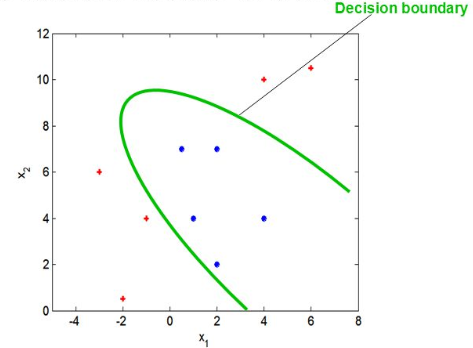
\includegraphics{images/db.png}

Classification is a process of finding the \textbf{decision boundary}
that best separate two classes
\end{frame}

\begin{frame}{Decision Boundary in Classification}
\phantomsection\label{decision-boundary-in-classification-1}
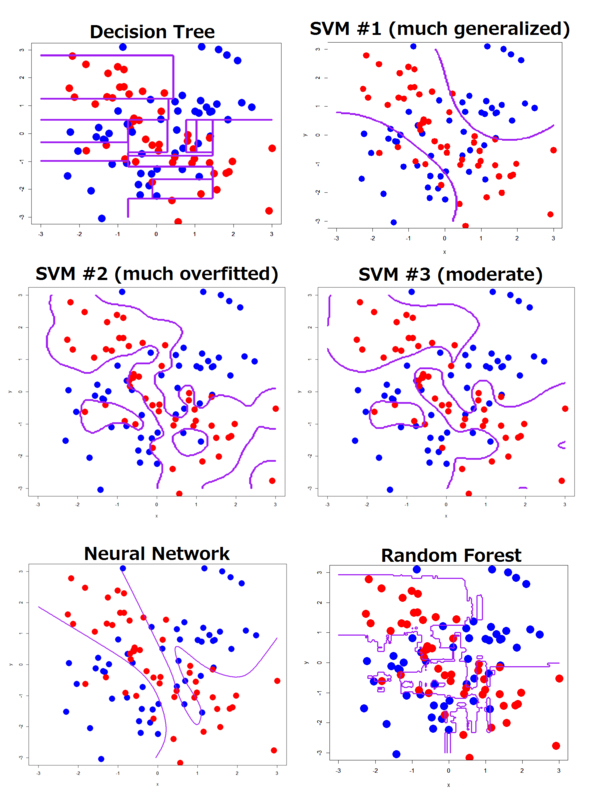
\includegraphics{images/db1.png}

SVM = Support Vector Machine
\end{frame}

\begin{frame}{Decision Tree}
\phantomsection\label{decision-tree}
\begin{itemize}
\tightlist
\item
  Decision Tree for classification is \textbf{Classification Tree}
\item
  Decision Tree for Regression is \textbf{Regression Tree}
\end{itemize}
\end{frame}

\begin{frame}{Example of Classification Tree}
\phantomsection\label{example-of-classification-tree}
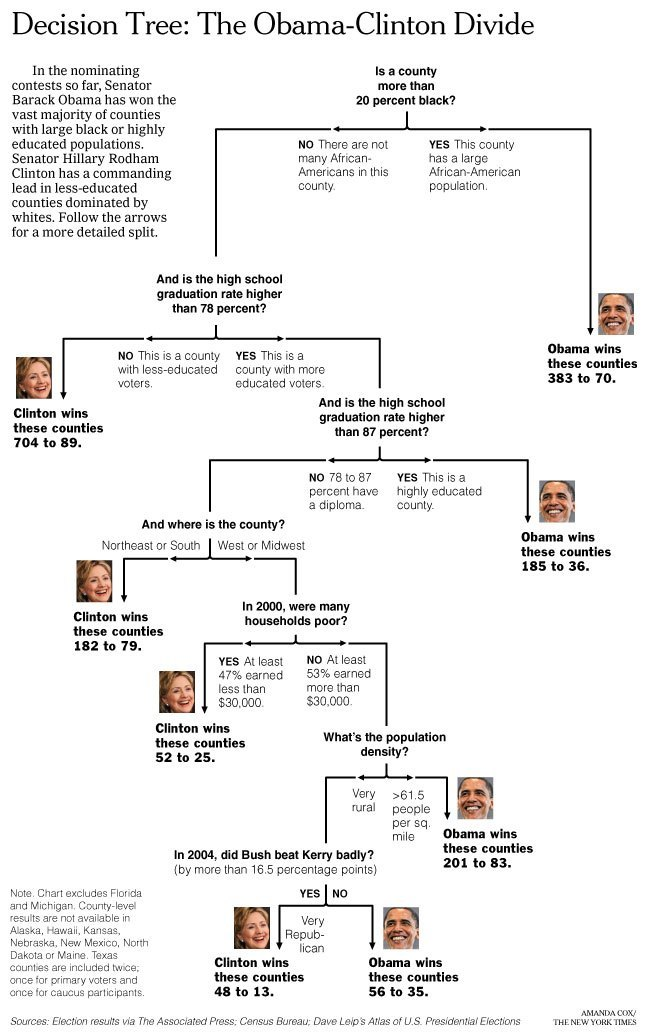
\includegraphics{images/tree2.jpg}

{[}Link{]}
(http://graphics8.nytimes.com/images/2008/04/16/us/0416-nat-subOBAMA.jpg)
\end{frame}

\begin{frame}{Classification Tree}
\phantomsection\label{classification-tree}
\begin{itemize}
\tightlist
\item
  In two dimension, classification Tree's decision boundary is a
  collection of horizontal and vertical line
\end{itemize}
\end{frame}

\begin{frame}{Data}
\phantomsection\label{data}
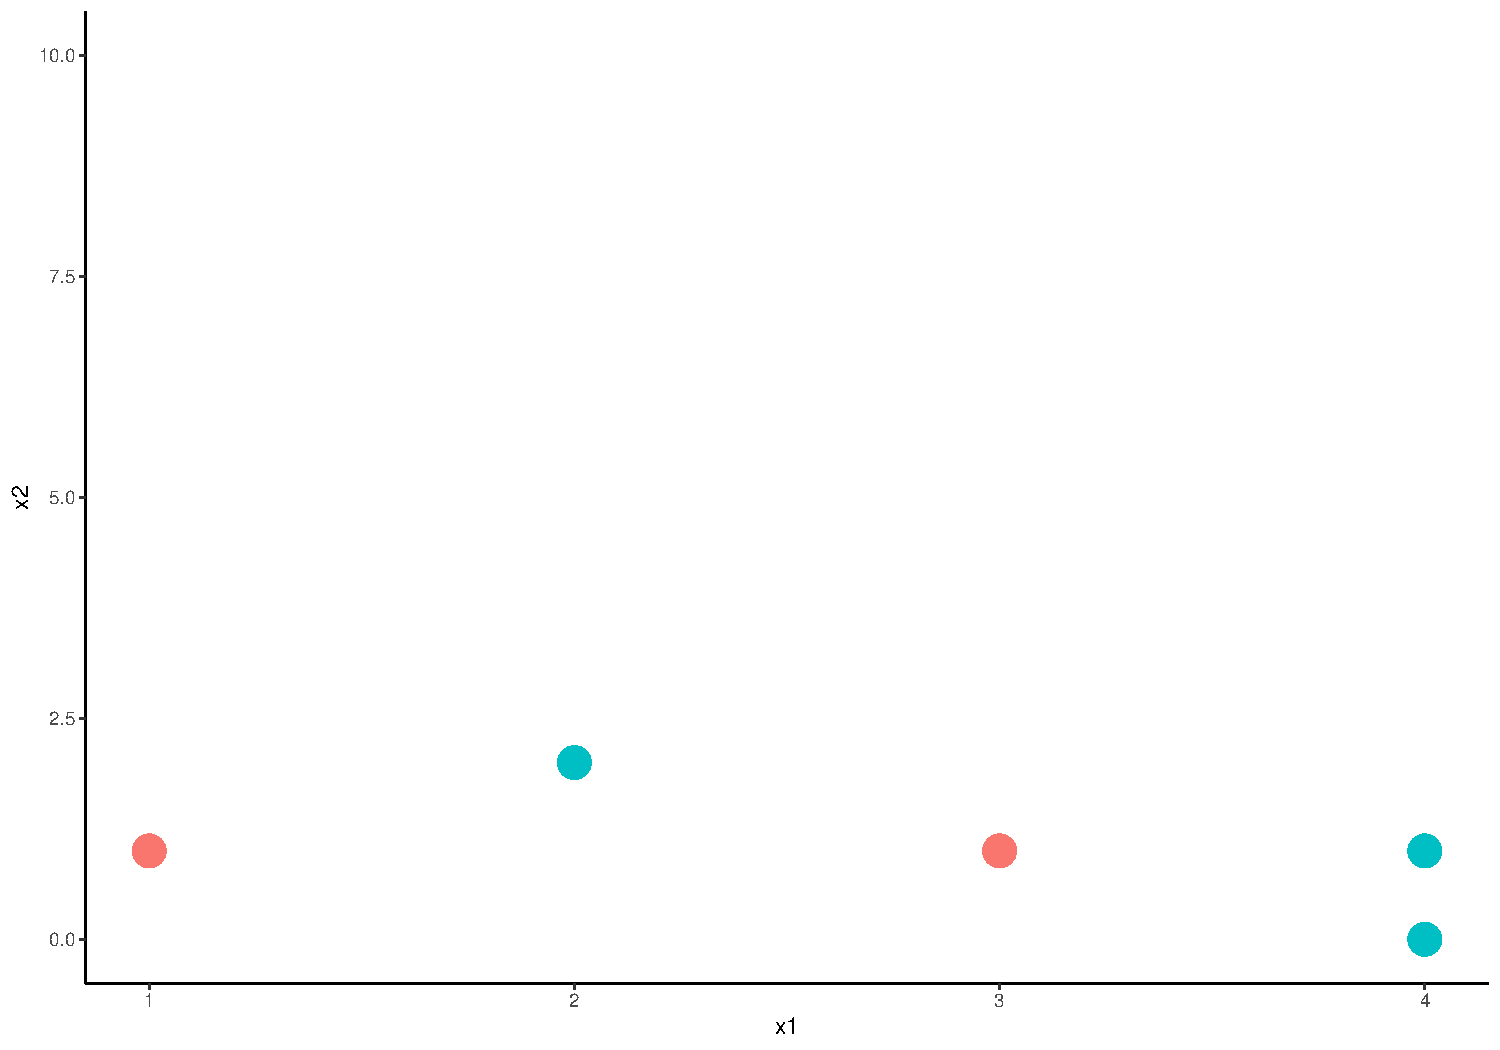
\includegraphics{fall24_classification_tree_remake_quarto_files/figure-beamer/unnamed-chunk-2-1.pdf}

\begin{itemize}
\tightlist
\item
  The tree starts by a vertical or horizontal line that \textbf{best}
  seperate the data
\item
  \textbf{Question}: Find a vertical line that best seperate
  \textbf{red} and \textbf{green}.
\end{itemize}
\end{frame}

\begin{frame}{One way to seperate the reds and greens}
\phantomsection\label{one-way-to-seperate-the-reds-and-greens}
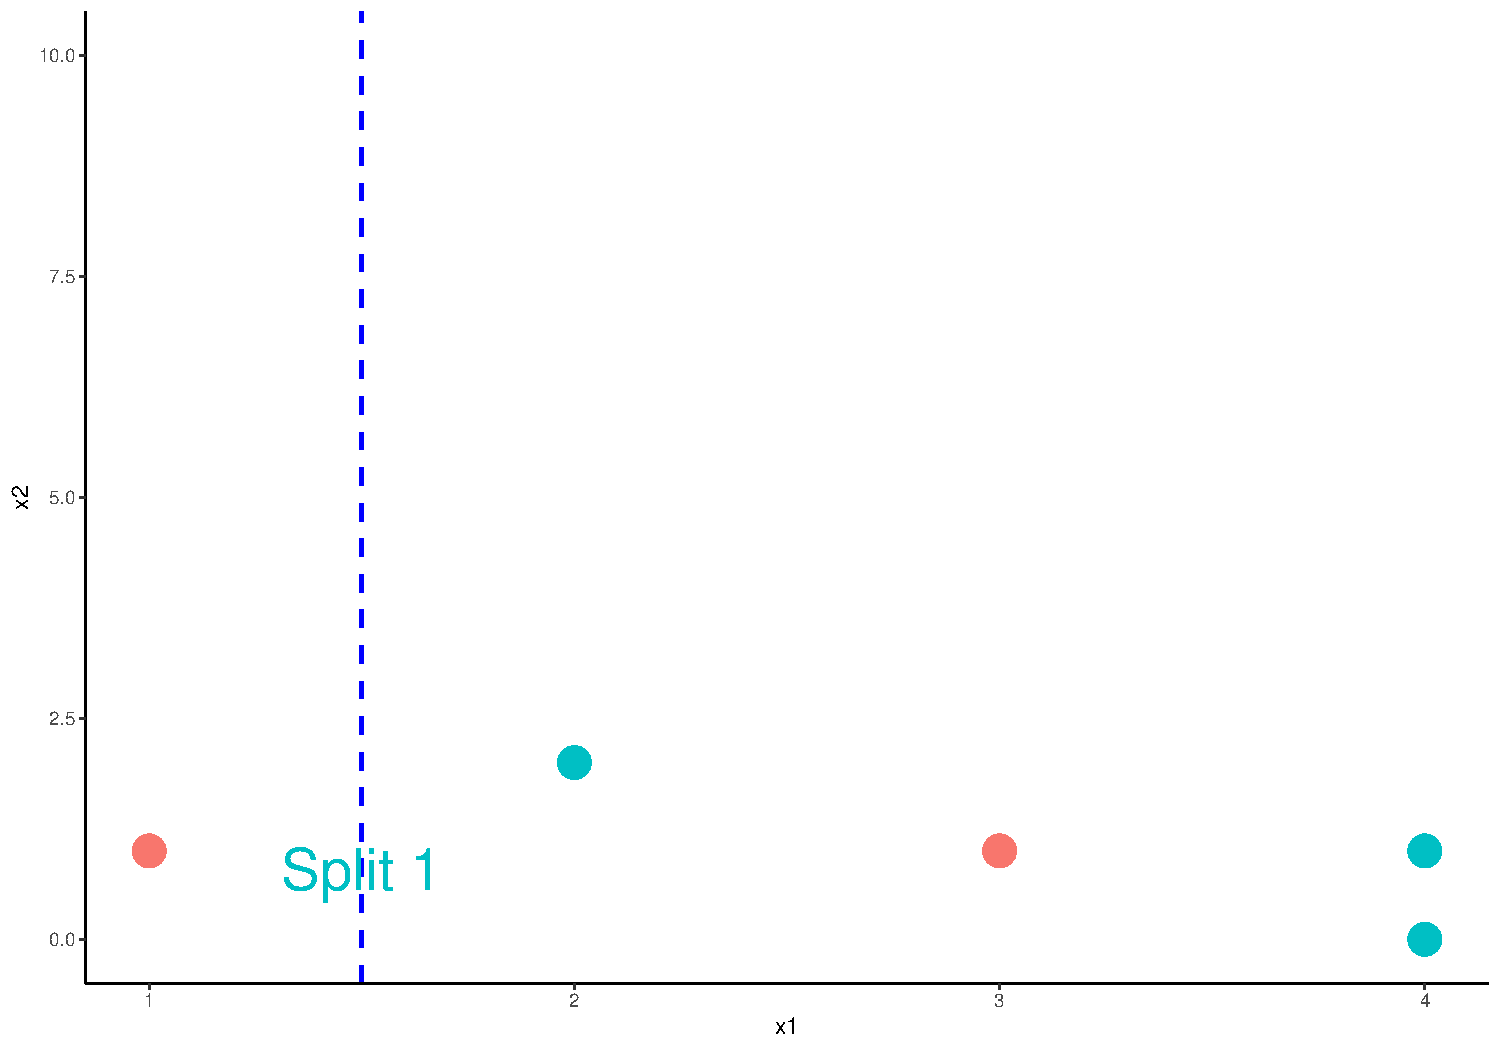
\includegraphics{fall24_classification_tree_remake_quarto_files/figure-beamer/unnamed-chunk-3-1.pdf}
\end{frame}

\begin{frame}{One way to seperate the reds and greens}
\phantomsection\label{one-way-to-seperate-the-reds-and-greens-1}
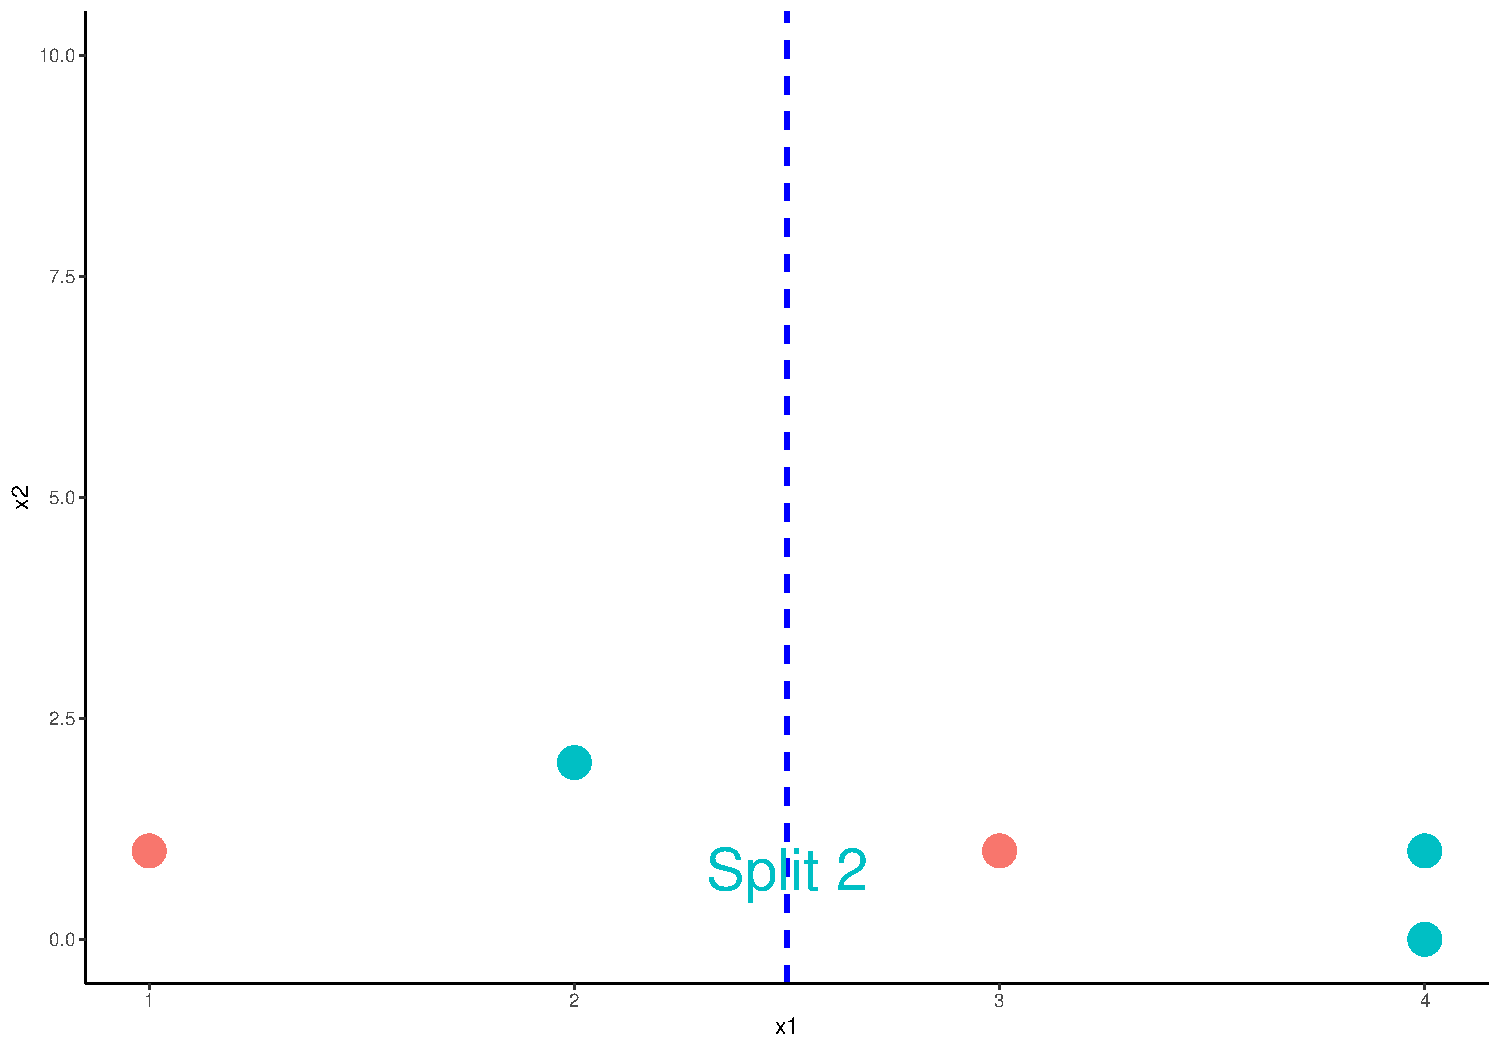
\includegraphics{fall24_classification_tree_remake_quarto_files/figure-beamer/unnamed-chunk-4-1.pdf}
\end{frame}

\begin{frame}{One way to seperate the reds and greens}
\phantomsection\label{one-way-to-seperate-the-reds-and-greens-2}
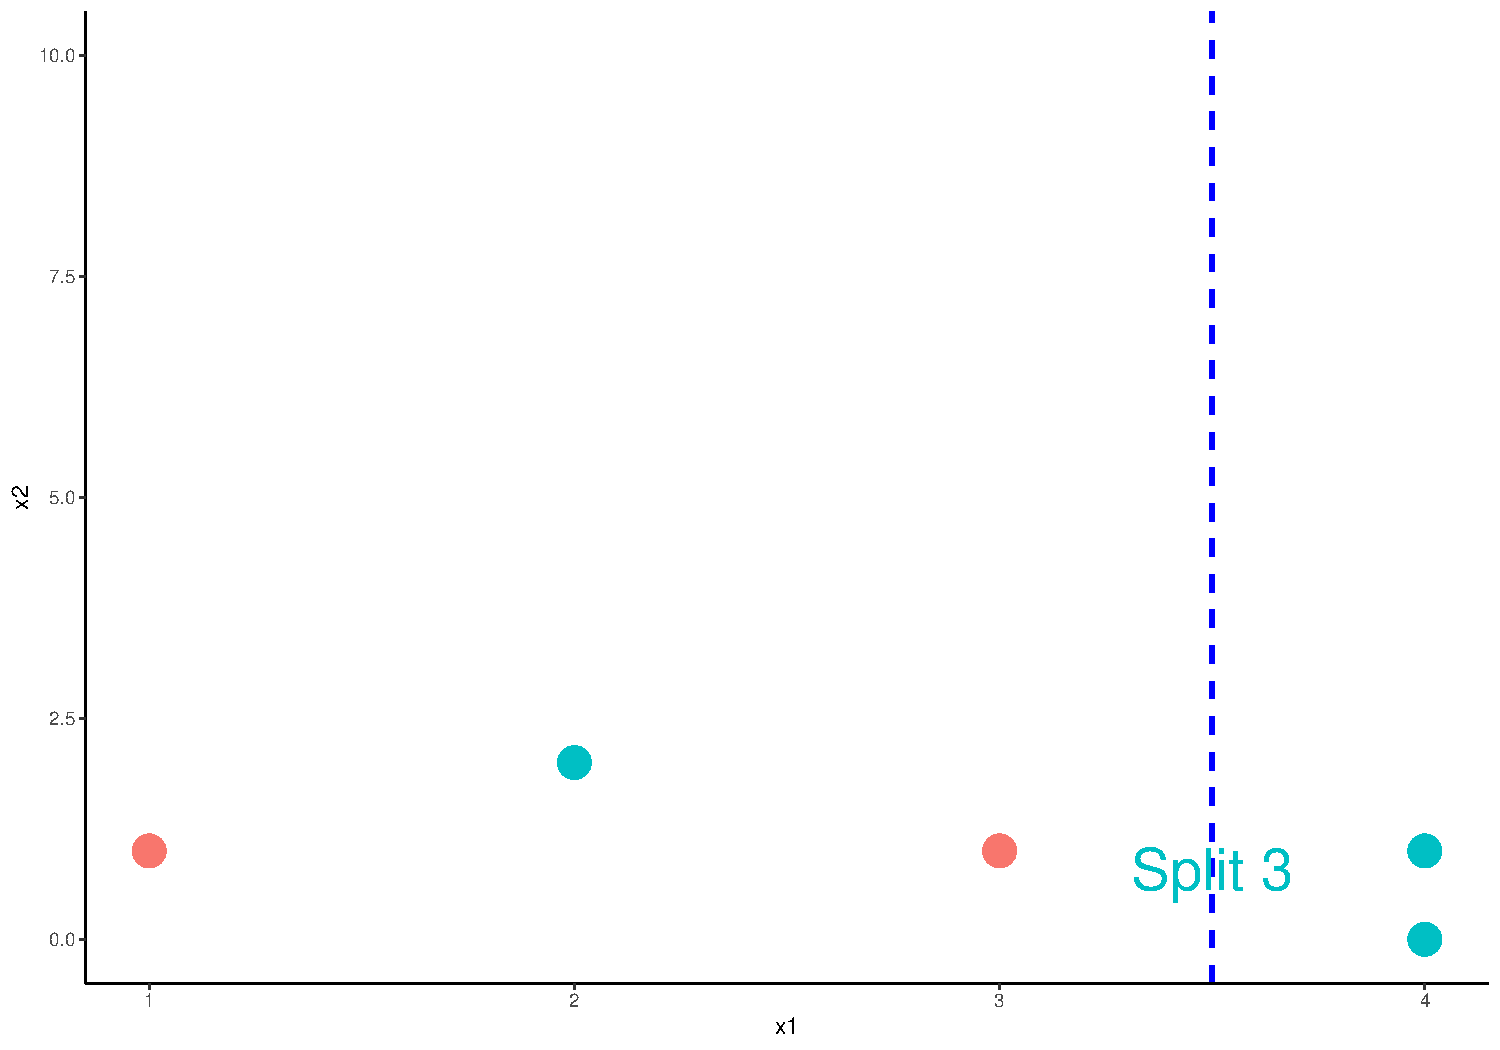
\includegraphics{fall24_classification_tree_remake_quarto_files/figure-beamer/unnamed-chunk-5-1.pdf}
\end{frame}

\begin{frame}{Question}
\phantomsection\label{question}
\begin{itemize}
\tightlist
\item
  \textbf{Question}: Which is the best split?
\end{itemize}
\end{frame}

\begin{frame}{Partial Answer}
\phantomsection\label{partial-answer}
\begin{itemize}
\tightlist
\item
  It looks like Split 1 and 3 are better than Split 2 since it
  misclassifies less
\item
  Which is the better split between Split 1 and Split 3?
\item
  We need to find a way to measure \emph{how good a split is}
\end{itemize}
\end{frame}

\begin{frame}{Impurity Measure}
\phantomsection\label{impurity-measure}
\begin{itemize}
\tightlist
\item
  The impurity of a node (\textbf{a node = a subset of the data or the
  original data}) measure how uncertain the node is.\\
\item
  For example, node A with 50\% reds and 50\% greens would be more
  uncertained than node B with 90\% reds and 10\% greens. Thus, node A
  has greater impurity than node B.
\item
  More uncertained \(=\) Greater impurity
\end{itemize}
\end{frame}

\begin{frame}{Impurity Measure}
\phantomsection\label{impurity-measure-1}
\begin{itemize}
\tightlist
\item
  A split that \emph{gains} more impurity is the \textbf{better split}!
\end{itemize}
\end{frame}

\begin{frame}{Impurity Gain}
\phantomsection\label{impurity-gain}
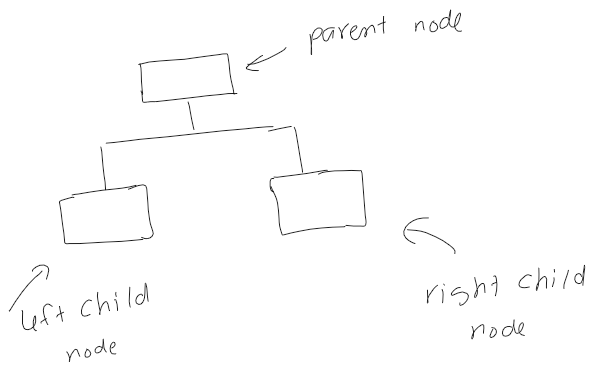
\includegraphics[width=\textwidth,height=1.5in]{images/parent_child.png}

\[
IG = I_{parent} - \frac{N_{left}}{N}I_{left}-\frac{N_{right}}{N}I_{right}
\]

\begin{itemize}
\tightlist
\item
  IG is Impurity Gain of the split
\item
  \(N_{left}\) and \(N_{right}\) are the number of points in the left
  child node and right child node, respectively.
\item
  \(N_{left}+N_{right}=N\)
\end{itemize}
\end{frame}

\begin{frame}{Impurity Measure}
\phantomsection\label{impurity-measure-2}
\begin{itemize}
\tightlist
\item
  Impurity can be measured by: classification error, Gini Index, and
  Entropy.
\end{itemize}
\end{frame}

\begin{frame}{Impurity Measure}
\phantomsection\label{impurity-measure-3}
\begin{itemize}
\tightlist
\item
  Let \(p_0\) and \(p_1\) be the proportion of class 0 and class 1 in a
  node.
\end{itemize}

\begin{align*}
{\text{By Classification Error: }} I &= min\{p_0, p_1\} \\
{\text{By Gini Index: }} I&= 1 - p_0^2-p_1^2 \\
{\text{By Entropy: }} I &= -p_0 \log_2(p_0)-p_1\log_2(p_1) 
\end{align*}
\end{frame}

\begin{frame}{Calculation}
\phantomsection\label{calculation}
\begin{itemize}
\tightlist
\item
  Let's calculate the impurity gain of the three splits to decide which
  split is the best
\end{itemize}
\end{frame}

\begin{frame}{IG By Classification Error}
\phantomsection\label{ig-by-classification-error}
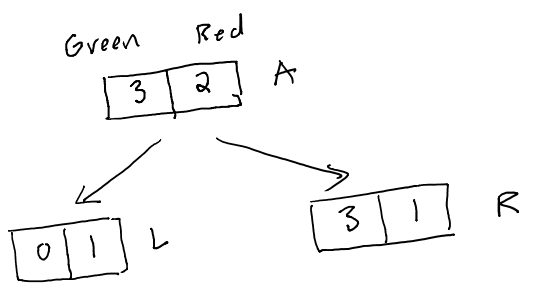
\includegraphics[width=\textwidth,height=1in]{images/im1.png}

\begin{itemize}
\tightlist
\item
  Let \textbf{green} and \textbf{red} be class 0 and class 1,
  respectively.
\end{itemize}

For Split 1: \(N = 5, N_{left} =1, N_{right} = 4\)

\begin{itemize}
\item
  Node \emph{parent,} A: \(p_0 = \frac{2}{5}, p_1 = \frac{3}{5}\). Thus,
  \(I_{A} = \text{min}(\frac{2}{5}, \frac{3}{5}) = \frac{2}{5}\)
\item
  Node \emph{child left,} L:
  \(p_0 = \frac{0}{1} = 0, p_1 = \frac{1}{1} = 1\). Thus,
  \(I_{L} = \text{min}(0, 1) = 0\)
\item
  Node \emph{child right,} R: \(p_0 = \frac{3}{4}, p_1 = \frac{1}{4}\).
  Thus, \(I_{R} = \text{min}(\frac{3}{4}, \frac{1}{4}) = \frac{1}{4}\)
\item
  Impurity Gain of Split 1:
\end{itemize}

\[IG = \frac{2}{5} - \frac{1}{5} \cdot 0-\frac{4}{5} \cdot \frac{1}{4} = 0.2\]
\end{frame}

\begin{frame}{IG By Classification Error}
\phantomsection\label{ig-by-classification-error-1}
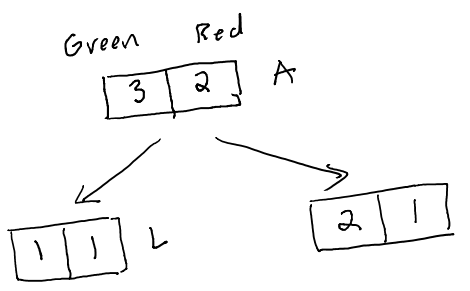
\includegraphics[width=\textwidth,height=1in]{images/im3.png}

For Split 2: \(N = 5, N_{left} =2, N_{right} = 3\)

\begin{itemize}
\item
  Node \emph{parent,} A: \(p_0 = \frac{2}{5}, p_1 = \frac{3}{5}\). Thus,
  \(I_{A} = \text{min}(\frac{2}{5}, \frac{3}{5}) = \frac{2}{5}\)
\item
  Node \emph{child left,} L: \(p_0 = \frac{1}{2}, p_1 = \frac{1}{2}\).
  Thus, \(I_{L} = \frac{1}{2}\)
\item
  Node \emph{child right,} R: \(p_0 = \frac{2}{3}, p_1 = \frac{1}{3}\).
  Thus, \(I_{R} = \text{min}(\frac{2}{3}, \frac{1}{3}) = \frac{1}{3}\)
\item
  Impurity Gain of Split 2:
\end{itemize}

\[IG = \frac{2}{5} - \frac{2}{5} \cdot \frac{1}{2}-\frac{3}{5} \cdot \frac{1}{3} = 0\]
\end{frame}

\begin{frame}{IG By Classification Error}
\phantomsection\label{ig-by-classification-error-2}
For Split 3: \(N = 5, N_{left} =3, N_{right} = 2\)

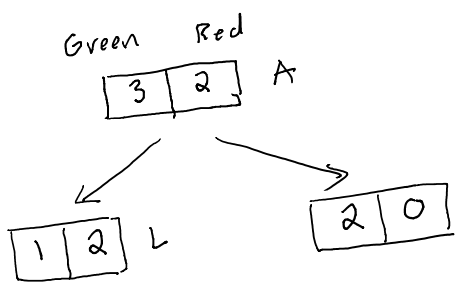
\includegraphics[width=\textwidth,height=1in]{images/im2.png}

\begin{itemize}
\item
  Node \emph{parent,} A: \(p_0 = \frac{2}{5}, p_1 = \frac{3}{5}\). Thus,
  \(I_{A} = \text{min}(\frac{2}{5}, \frac{3}{5}) = \frac{2}{5}\)
\item
  Node \emph{child left,} L: \(p_0 = \frac{1}{3}, p_1 = \frac{2}{3}\).
  Thus, \(I_{A} = \text{min}(\frac{1}{3}, \frac{2}{3}) = \frac{1}{3}\)
\item
  Node \emph{child right,} R: \(p_0 = \frac{2}{2}, p_1 = \frac{0}{2}\).
  Thus, \(I_{R} = \text{min}(1,0) = 0\)
\item
  Impurity Gain of Split 3:
\end{itemize}

\[IG = \frac{2}{5} - \frac{3}{5} \cdot \frac{1}{3}-\frac{2}{5} \cdot 0 = 0.2\]
\end{frame}

\begin{frame}{Comparing IG By Classification Error}
\phantomsection\label{comparing-ig-by-classification-error}
\begin{longtable}[]{@{}ll@{}}
\toprule\noalign{}
Split & IG \\
\midrule\noalign{}
\endhead
1 & 0.2 \\
2 & 0 \\
3 & 0.2 \\
\bottomrule\noalign{}
\end{longtable}

\begin{itemize}
\tightlist
\item
  By classification error, Split 1 and Split 3 are tie as the best
  because they have the same impurity gain.
\end{itemize}
\end{frame}

\begin{frame}{IG By Gini Index}
\phantomsection\label{ig-by-gini-index}
For Split 1: \(N = 5, N_{left} =1, N_{right} = 4\)

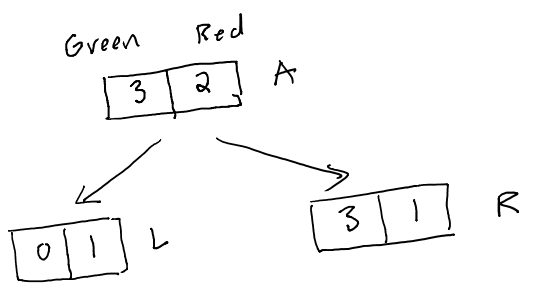
\includegraphics[width=\textwidth,height=1in]{images/im1.png}

\begin{itemize}
\item
  Node \emph{parent,} A: \(p_0 = \frac{2}{5}, p_1 = \frac{3}{5}\). Thus,
  \(I_{A} = 1 - (\frac{2}{5})^2-(\frac{3}{5})^2 = 0.48\)
\item
  Node \emph{child left,} L:
  \(p_0 = \frac{0}{1} = 0, p_1 = \frac{1}{1} = 1\). Thus,
  \[I_{L} = 1 -0^2-1^2 = 0\]
\item
  Node \emph{child right,} R: \(p_0 = \frac{3}{4}, p_1 = \frac{1}{4}\).
  Thus, \[I_{R} = 1-(\frac{3}{4})^2-(\frac{1}{4})^2 = 0.375\]
\item
  Impurity Gain of Split 1:
\end{itemize}

\[IG = 0.48 - \frac{1}{5} \cdot 0-\frac{4}{5} \cdot 0.375 = 0.18\] \#\#
IG By Gini Index

For Split 2: \(N = 5, N_{left} =2, N_{right} = 3\)

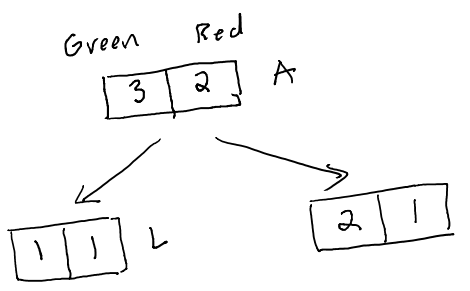
\includegraphics{images/im3.png}\{1.5in\}

\begin{itemize}
\item
  Node \emph{parent,} A: \(p_0 = \frac{2}{5}, p_1 = \frac{3}{5}\). Thus,
  \(I_{A} = 1-(\frac{2}{5})^2- (\frac{3}{5})^2 = 0.48\)
\item
  Node \emph{child left,} L: \(p_0 = \frac{1}{2}, p_1 = \frac{1}{2}\).
  Thus, \(I_{L} = 1- (\frac{1}{2})^2-(\frac{1}{2})^2=0.5\)
\item
  Node \emph{child right,} R: \(p_0 = \frac{2}{3}, p_1 = \frac{1}{3}\).
  Thus, \(I_{R} = 1-(\frac{2}{3})^2 -(\frac{1}{3})^2 = 0.44\)
\item
  Impurity Gain of Split 2:
\end{itemize}

\[IG = 0.48 - \frac{2}{5} \cdot \frac{1}{2}-\frac{3}{5} \cdot 0.44 = 0.016\]
\end{frame}

\begin{frame}{IG By Gini Index}
\phantomsection\label{ig-by-gini-index-1}
For Split 3: \(N = 5, N_{left} =3, N_{right} = 2\)

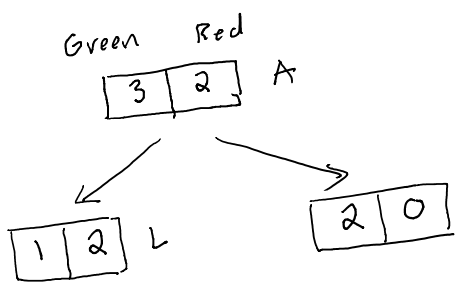
\includegraphics{images/im2.png}\{1.5in\}

\begin{itemize}
\item
  Node \emph{parent,} A: \(I_{A} = 0.48\)
\item
  Node \emph{child left,} L: \(p_0 = \frac{1}{3}, p_1 = \frac{2}{3}\).
  Thus, \(I_{A} = 1-(\frac{1}{3})^2 -(\frac{2}{3})^2 = 0.44\)
\item
  Node \emph{child right,} R: \(p_0 = \frac{2}{2}, p_1 = \frac{0}{2}\).
  Thus, \(I_{R} = 1-0^2-1^2 = 0\)
\item
  Impurity Gain of Split 3:
\end{itemize}

\[IG = 0.48 - \frac{3}{5} \cdot 0.44 - \frac{2}{5} \cdot 0 = 0.216\]
\end{frame}

\begin{frame}{Comparing IG By Gini Index}
\phantomsection\label{comparing-ig-by-gini-index}
\begin{longtable}[]{@{}ll@{}}
\toprule\noalign{}
& IG \\
\midrule\noalign{}
\endhead
Split 1 & 0.18 \\
Split 2 & 0.016 \\
Split 3 & 0.216 \\
\bottomrule\noalign{}
\end{longtable}

\begin{itemize}
\tightlist
\item
  By Gini Index, Split 3 is the best because it has the greatest
  impurity gain.
\end{itemize}
\end{frame}

\begin{frame}{IG By Entropy}
\phantomsection\label{ig-by-entropy}
For Split 1: \(N = 5, N_{left} =1, N_{right} = 4\)

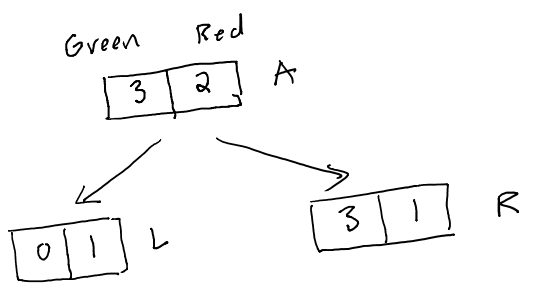
\includegraphics{images/im1.png}\{1.5in\}

\begin{itemize}
\item
  Node \emph{parent,} A: \(p_0 = \frac{2}{5}, p_1 = \frac{3}{5}\). Thus,
  \(I_{A} = - log_2(\frac{2}{5})-log_2(\frac{3}{5}) = 0.971\)
\item
  Node \emph{child left,} L:
  \(p_0 = \frac{0}{1} = 0, p_1 = \frac{1}{1} = 1\). Thus, \(I_{L} = 0\)
\item
  Node \emph{child right,} R: \(p_0 = \frac{3}{4}, p_1 = \frac{1}{4}\).
  Thus, \[I_{R} = -log_2(\frac{3}{4})-log_2(\frac{1}{4}) = 0.811\]
\item
  Impurity Gain of Split 1:
\end{itemize}

\[IG = 0.971 - \frac{1}{5} \cdot 0-\frac{4}{5} \cdot 0.811 = 0.322\]
\end{frame}

\begin{frame}{IG By Entropy}
\phantomsection\label{ig-by-entropy-1}
For Split 2: \(N = 5, N_{left} =2, N_{right} = 3\)

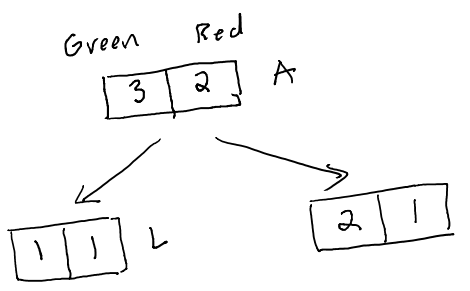
\includegraphics{images/im3.png}

\begin{itemize}
\item
  Node \emph{parent,} A: \(p_0 = \frac{2}{5}, p_1 = \frac{3}{5}\). Thus,
  \(I_{A} = 0.971\)
\item
  Node \emph{child left,} L: \(p_0 = \frac{1}{2}, p_1 = \frac{1}{2}\).
  Thus, \(I_{L} = - log_1(\frac{1}{2})-log_2(\frac{1}{2})=1\)
\item
  Node \emph{child right,} R: \(p_0 = \frac{2}{3}, p_1 = \frac{1}{3}\).
  Thus, \(I_{R} = -log_2(\frac{2}{3}) -log_2(\frac{1}{3}) = 0.918\)
\item
  Impurity Gain of Split 2:
\end{itemize}

\[IG = 0.971 - \frac{2}{5} \cdot 1-\frac{3}{5} \cdot 0.918 = 0.02\]
\end{frame}

\begin{frame}{IG By Entropy}
\phantomsection\label{ig-by-entropy-2}
For Split 3: \(N = 5, N_{left} =3, N_{right} = 2\)

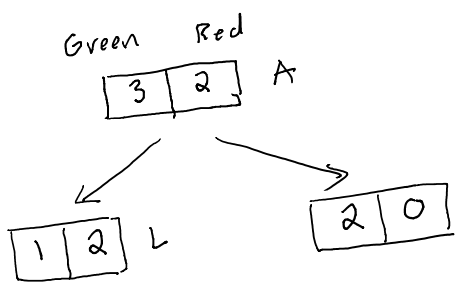
\includegraphics{images/im2.png}

\begin{itemize}
\item
  Node \emph{parent,} A: \(I_{A} = 0.971\)
\item
  Node \emph{child left,} L: \(p_0 = \frac{1}{3}, p_1 = \frac{2}{3}\).
  Thus, \(I_{A} = -log_2(\frac{1}{3}) -log_2(\frac{2}{3}) = 0.918\)
\item
  Node \emph{child right,} R: \(p_0 = \frac{2}{2}, p_1 = \frac{0}{2}\).
  Thus, \(I_{R} = 0\)
\item
  Impurity Gain of Split 3:
\end{itemize}

\[IG = 0.971 - \frac{3}{5} \cdot 0.918 - \frac{2}{5} \cdot 0 = 0.42\]
\end{frame}

\begin{frame}{Comparing IG By Entropy}
\phantomsection\label{comparing-ig-by-entropy}
\begin{longtable}[]{@{}ll@{}}
\toprule\noalign{}
& IG \\
\midrule\noalign{}
\endhead
Split 1 & 0.322 \\
Split 2 & 0.02 \\
Split 3 & 0.42 \\
\bottomrule\noalign{}
\end{longtable}

\begin{itemize}
\tightlist
\item
  By Gini Index, Split 3 is the best because it has the greatest
  impurity gain.
\end{itemize}
\end{frame}

\begin{frame}{Comparing Impurity Measures}
\phantomsection\label{comparing-impurity-measures}
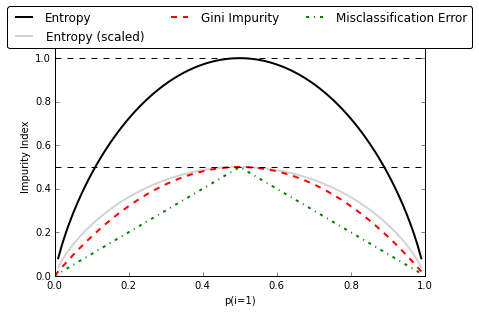
\includegraphics{images/i.png} - Relation between impurity and the class
probabilities. All impurity measures are maximized at \(p_1 =1/2\) and
minimized at \(p_1 = 0\) and \(p_1=1\).
\end{frame}

\begin{frame}{Another Example}
\phantomsection\label{another-example}
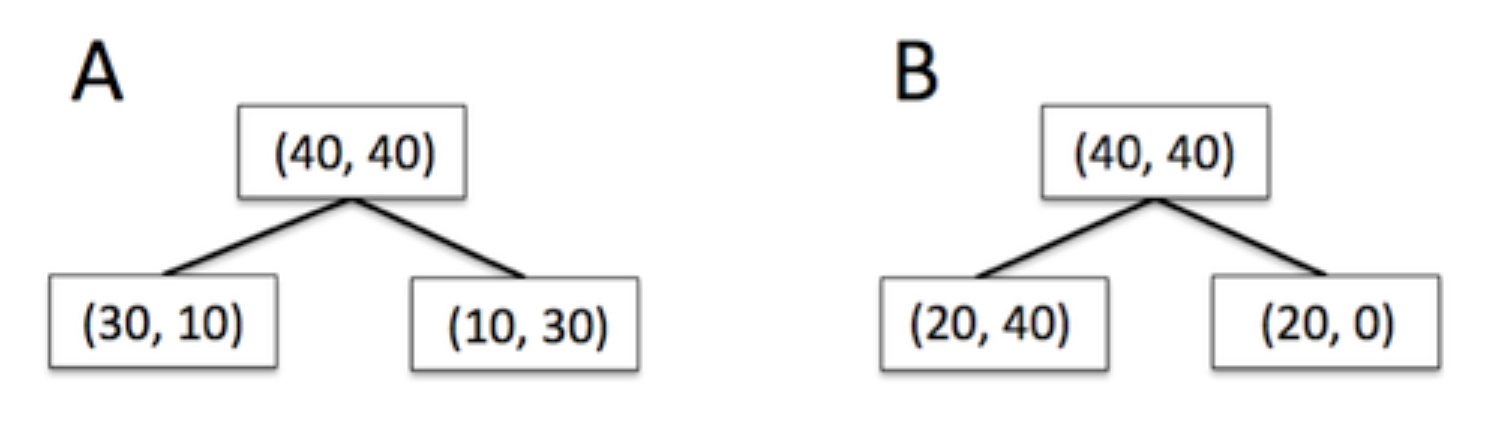
\includegraphics{images/i1.png} - Which split is better?
\end{frame}

\begin{frame}{Decide the best split using Chi-Square test of
Independence}
\phantomsection\label{decide-the-best-split-using-chi-square-test-of-independence}
\begin{itemize}
\tightlist
\item
  Besides impurity gain, one can use the Chi-square, \(\chi^2\), test of
  independence to decide the best split.
\end{itemize}
\end{frame}

\begin{frame}{Review of Chi-Square test of Independence}
\phantomsection\label{review-of-chi-square-test-of-independence}
\begin{itemize}
\tightlist
\item
  Let \(X\) and \(Y\) be two categorical variables.
\item
  We want to test if \(X\) and \(Y\) are independent/associated

  \begin{itemize}
  \tightlist
  \item
    \(H_0\): \(X\) and \(Y\) are independent
  \item
    \(H_{\alpha}:\) \(X\) and \(Y\) are dependent
  \end{itemize}
\item
  Test statistic:
\end{itemize}

\[\sum\frac{(e_i-o_i)^2}{e_i} \sim \chi^2 \text{ distribution with degree of freedom} (n-1)(m-1)\]
\end{frame}

\begin{frame}{Review of Chi-Square test of Independence}
\phantomsection\label{review-of-chi-square-test-of-independence-1}
\begin{itemize}
\tightlist
\item
  In our context, the greater the \(\chi^2\) value, the smaller the
  \(p-value\)
\item
  The smaller the \(p-value\), the more dependent the two variables are.
  Thus the better the split is.
\item
  Therefore, we look for the split with the \textbf{greatest} \(\chi^2\)
  value.
\end{itemize}
\end{frame}

\begin{frame}{Applying to Our Example}
\phantomsection\label{applying-to-our-example}
\begin{itemize}
\tightlist
\item
  We will calculate the \(\chi^2\) values of the three splits.\\
\item
  The best split is the split with the greatest \(\chi^2\) value.
\end{itemize}
\end{frame}

\begin{frame}{Split 1}
\phantomsection\label{split-1}
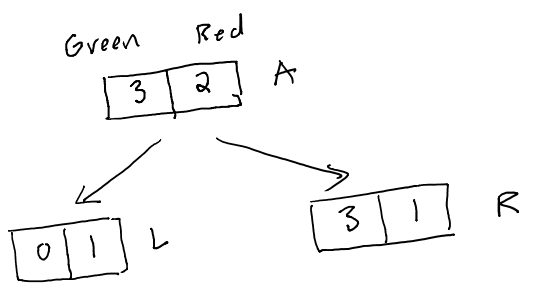
\includegraphics{images/im1.png}

\begin{longtable}[]{@{}llll@{}}
\toprule\noalign{}
& Greens & Reds & \\
\midrule\noalign{}
\endhead
Left Branch & 0 (Cell 1) & 1 (Cell 2) & 1 \\
Right Branch & 3 (Cell 3) & 1 (Cell 4) & 4 \\
& 3 & 2 & \\
\bottomrule\noalign{}
\end{longtable}

\[\chi^2 = \frac{(e_1-o_1)^2}{e_1}+\frac{(e_2-o_2)^2}{e_2}+\frac{(e_3-o_3)^2}{e_3}+\frac{(e_4-o_4)^2}{e_4}\]

\begin{itemize}
\item
  \(i=1\) (Cell 1): \(e_1 = \frac{1\cdot 3}{5}\), \(o_1 = 0\)
\item
  \(i=2\) (Cell 2): \(e_2 = \frac{1\cdot 2}{5}\), \(o_2 = 1\)
\item
  \(i=3\) (Cell 3): \(e_3 = \frac{3\cdot 4}{5}\), \(o_3 = 3\)
\item
  \(i=4\) (Cell 4): \(e_4 = \frac{2\cdot 4}{5}\), \(o_4 = 1\)
\item
  Plug in, we have: \[\chi^2 = 1.875\]
\end{itemize}
\end{frame}

\begin{frame}{Split 2}
\phantomsection\label{split-2}
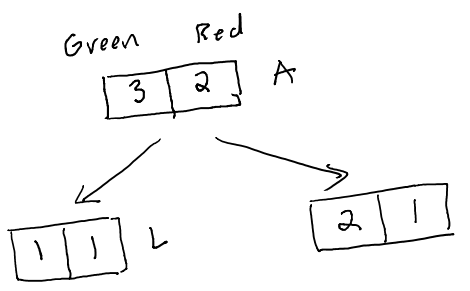
\includegraphics{images/im3.png}

\begin{longtable}[]{@{}llll@{}}
\toprule\noalign{}
& Greens & Reds & \\
\midrule\noalign{}
\endhead
Left Branch & 1 (Cell 1) & 1 (Cell 2) & 2 \\
Right Branch & 2 (Cell 3) & 1 (Cell 4) & 3 \\
& 3 & 2 & \\
\bottomrule\noalign{}
\end{longtable}

\[\chi^2 = \frac{(e_1-o_1)^2}{e_1}+\frac{(e_2-o_2)^2}{e_2}+\frac{(e_3-o_3)^2}{e_3}+\frac{(e_4-o_4)^2}{e_4}\]

\begin{itemize}
\item
  \(i=1\) (Cell 1): \(e_1 = \frac{2\cdot 3}{5}\), \(o_1 = 1\)
\item
  \(i=2\) (Cell 2): \(e_2 = \frac{2\cdot 2}{5}\), \(o_2 = 1\)
\item
  \(i=3\) (Cell 3): \(e_3 = \frac{3\cdot 3}{5}\), \(o_3 = 2\)
\item
  \(i=4\) (Cell 4): \(e_4 = \frac{3\cdot 2}{5}\), \(o_4 = 1\)
\item
  Plug in, we have: \[\chi^2 = 0.139\]
\end{itemize}
\end{frame}

\begin{frame}{Split 3}
\phantomsection\label{split-3}
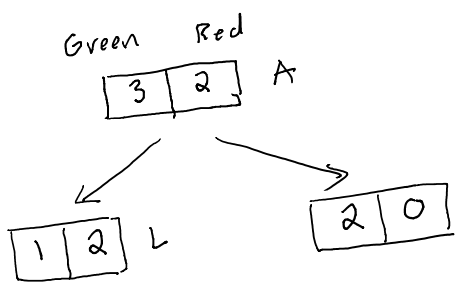
\includegraphics{images/im2.png}

\begin{longtable}[]{@{}llll@{}}
\toprule\noalign{}
& Greens & Reds & \\
\midrule\noalign{}
\endhead
Left Branch & 1 (Cell 1) & 2 (Cell 2) & 3 \\
Right Branch & 2 (Cell 3) & 0 (Cell 4) & 2 \\
& 3 & 2 & \\
\bottomrule\noalign{}
\end{longtable}

\[\chi^2 = \frac{(e_1-o_1)^2}{e_1}+\frac{(e_2-o_2)^2}{e_2}+\frac{(e_3-o_3)^2}{e_3}+\frac{(e_4-o_4)^2}{e_4}\]

\begin{itemize}
\item
  (Cell 1): \(e_1 = \frac{2\cdot 3}{5}\), \(o_1 = 1\)
\item
  (Cell 2): \(e_2 = \frac{2\cdot 2}{5}\), \(o_2 = 2\)
\item
  (Cell 3): \(e_3 = \frac{3\cdot 3}{5}\), \(o_3 = 2\)
\item
  (Cell 4): \(e_4 = \frac{3\cdot 2}{5}\), \(o_4 = 0\)
\item
  Plug in, we have: \[\chi^2 = 2.222\]
\end{itemize}
\end{frame}

\begin{frame}{Comparing the three splits}
\phantomsection\label{comparing-the-three-splits}
\begin{longtable}[]{@{}ll@{}}
\toprule\noalign{}
& \(\chi^2\) \\
\midrule\noalign{}
\endhead
Split 1 & 1.875 \\
Split 2 & 0.139 \\
Split 3 & 2.222 \\
\bottomrule\noalign{}
\end{longtable}

\begin{itemize}
\tightlist
\item
  Split 3 is the best because it has the greatest \(\chi^2\)!
\end{itemize}
\end{frame}

\begin{frame}{Logworth}
\phantomsection\label{logworth}
\begin{itemize}
\tightlist
\item
  The quality of the split can be measured by \textbf{Logworth}
\item
  Formula: \[logworth = -log(p\text{_}value)\]
\item
  The greater the logworth, the better the split
\end{itemize}
\end{frame}

\begin{frame}{Logworth}
\phantomsection\label{logworth-1}
\begin{longtable}[]{@{}llll@{}}
\toprule\noalign{}
& \(\chi^2\) & p-value & logworth \\
\midrule\noalign{}
\endhead
Split 1 & 1.875 & 0.114 & 0.943 \\
Split 2 & 0.139 & 0.998 & 0.0008 \\
Split 3 & 2.222 & 0.088 & 1.055 \\
\bottomrule\noalign{}
\end{longtable}

\begin{itemize}
\item
  Greatest \(\chi^2\) = Lowest \(p-value\) = Greatest logworth = Best
  Split
\item
  Split 3 is the best split!
\end{itemize}
\end{frame}

\begin{frame}{What happens after the first split?}
\phantomsection\label{what-happens-after-the-first-split}
\begin{itemize}
\tightlist
\item
  After the first split, the data are divided into to subsets.
\item
  The splitting process is repeated for each subset.
\item
  The process ends when a stopping criteria is satisfied
\end{itemize}
\end{frame}

\begin{frame}{Stopping Criteria}
\phantomsection\label{stopping-criteria}
\begin{itemize}
\tightlist
\item
  Minimum Leaf Size: The minimum of observations in the leaves
\item
  Maximum Number of Leaves
\item
  Maximum Depth
\item
  Others
\end{itemize}
\end{frame}

\begin{frame}{Stopping Criteria}
\phantomsection\label{stopping-criteria-1}
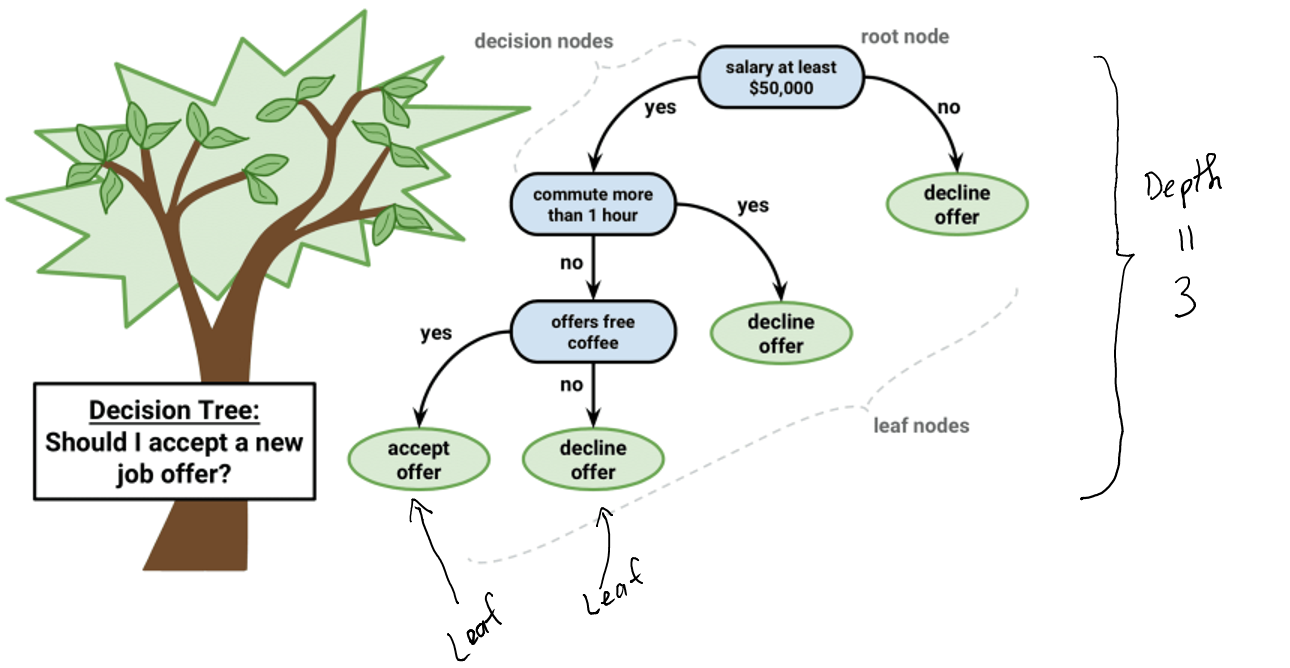
\includegraphics{images/tree6.png}
\end{frame}

\begin{frame}{Decision Tree Algorithm - How to grow a tree}
\phantomsection\label{decision-tree-algorithm---how-to-grow-a-tree}
\begin{itemize}
\tightlist
\item
  Step 1: Calculate the impurity gain or \(p-value\) of all possible
  splits at all variables
\item
  Step 2: Select the split that give the maximum impurity gain or lowest
  \(p-value\) to split the data into two subdata \(D_1\) and \(D_2\)
\item
  Repeat \emph{Step 1} and \emph{Step 2} to both \(D_1\) and \(D_2\).
\item
  Until a stopping criteria is satisfied
\end{itemize}
\end{frame}

\begin{frame}{Complexity of Decision Tree}
\phantomsection\label{complexity-of-decision-tree}
\begin{itemize}
\tightlist
\item
  A complexity of a tree can be measured by the number of leaves the
  tree has
\item
  The more leaves a tree has, the more complex the tree is.
\item
  A complex tree may be \textbf{overfitted}, i.e.~having low training
  error but high testing error.
\end{itemize}
\end{frame}

\begin{frame}{Prunning a tree}
\phantomsection\label{prunning-a-tree}
\begin{itemize}
\tightlist
\item
  For any given data, one can construct a tree that achives 0
  misclassification on training data
\item
  After growing the tree one needs to prune it to avoid overfittted
\end{itemize}
\end{frame}

\begin{frame}{Prunning a tree}
\phantomsection\label{prunning-a-tree-1}
\begin{itemize}
\tightlist
\item
  The tree with maximum number of leaves is called the \textbf{maximal
  tree} (still satisfied the stopping rule)
\item
  From the \textbf{maximal tree}, leaves are cut down, one by one, to
  obatined all possible subtrees
\item
  The subtree with lowest error on validation data, is the
  \textbf{optimal tree}
\end{itemize}
\end{frame}

\begin{frame}{Maximal vs Optimal Tree}
\phantomsection\label{maximal-vs-optimal-tree}
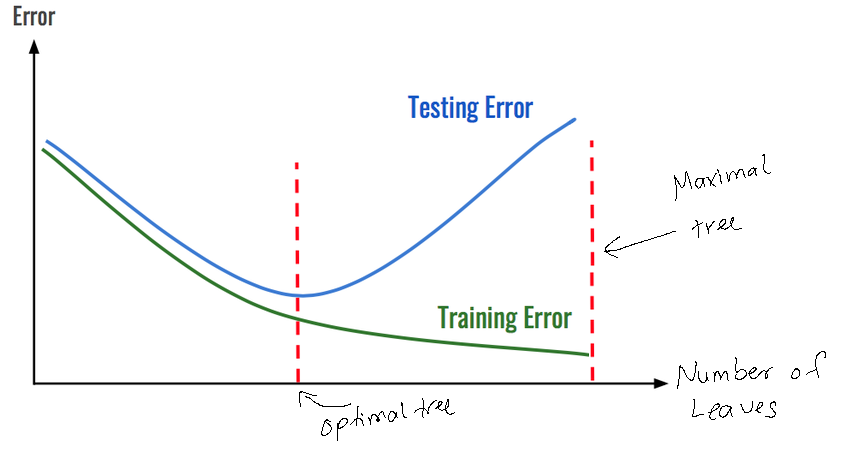
\includegraphics{images/tree7.png}
\end{frame}

\begin{frame}{Example of Tree Prunning}
\phantomsection\label{example-of-tree-prunning}
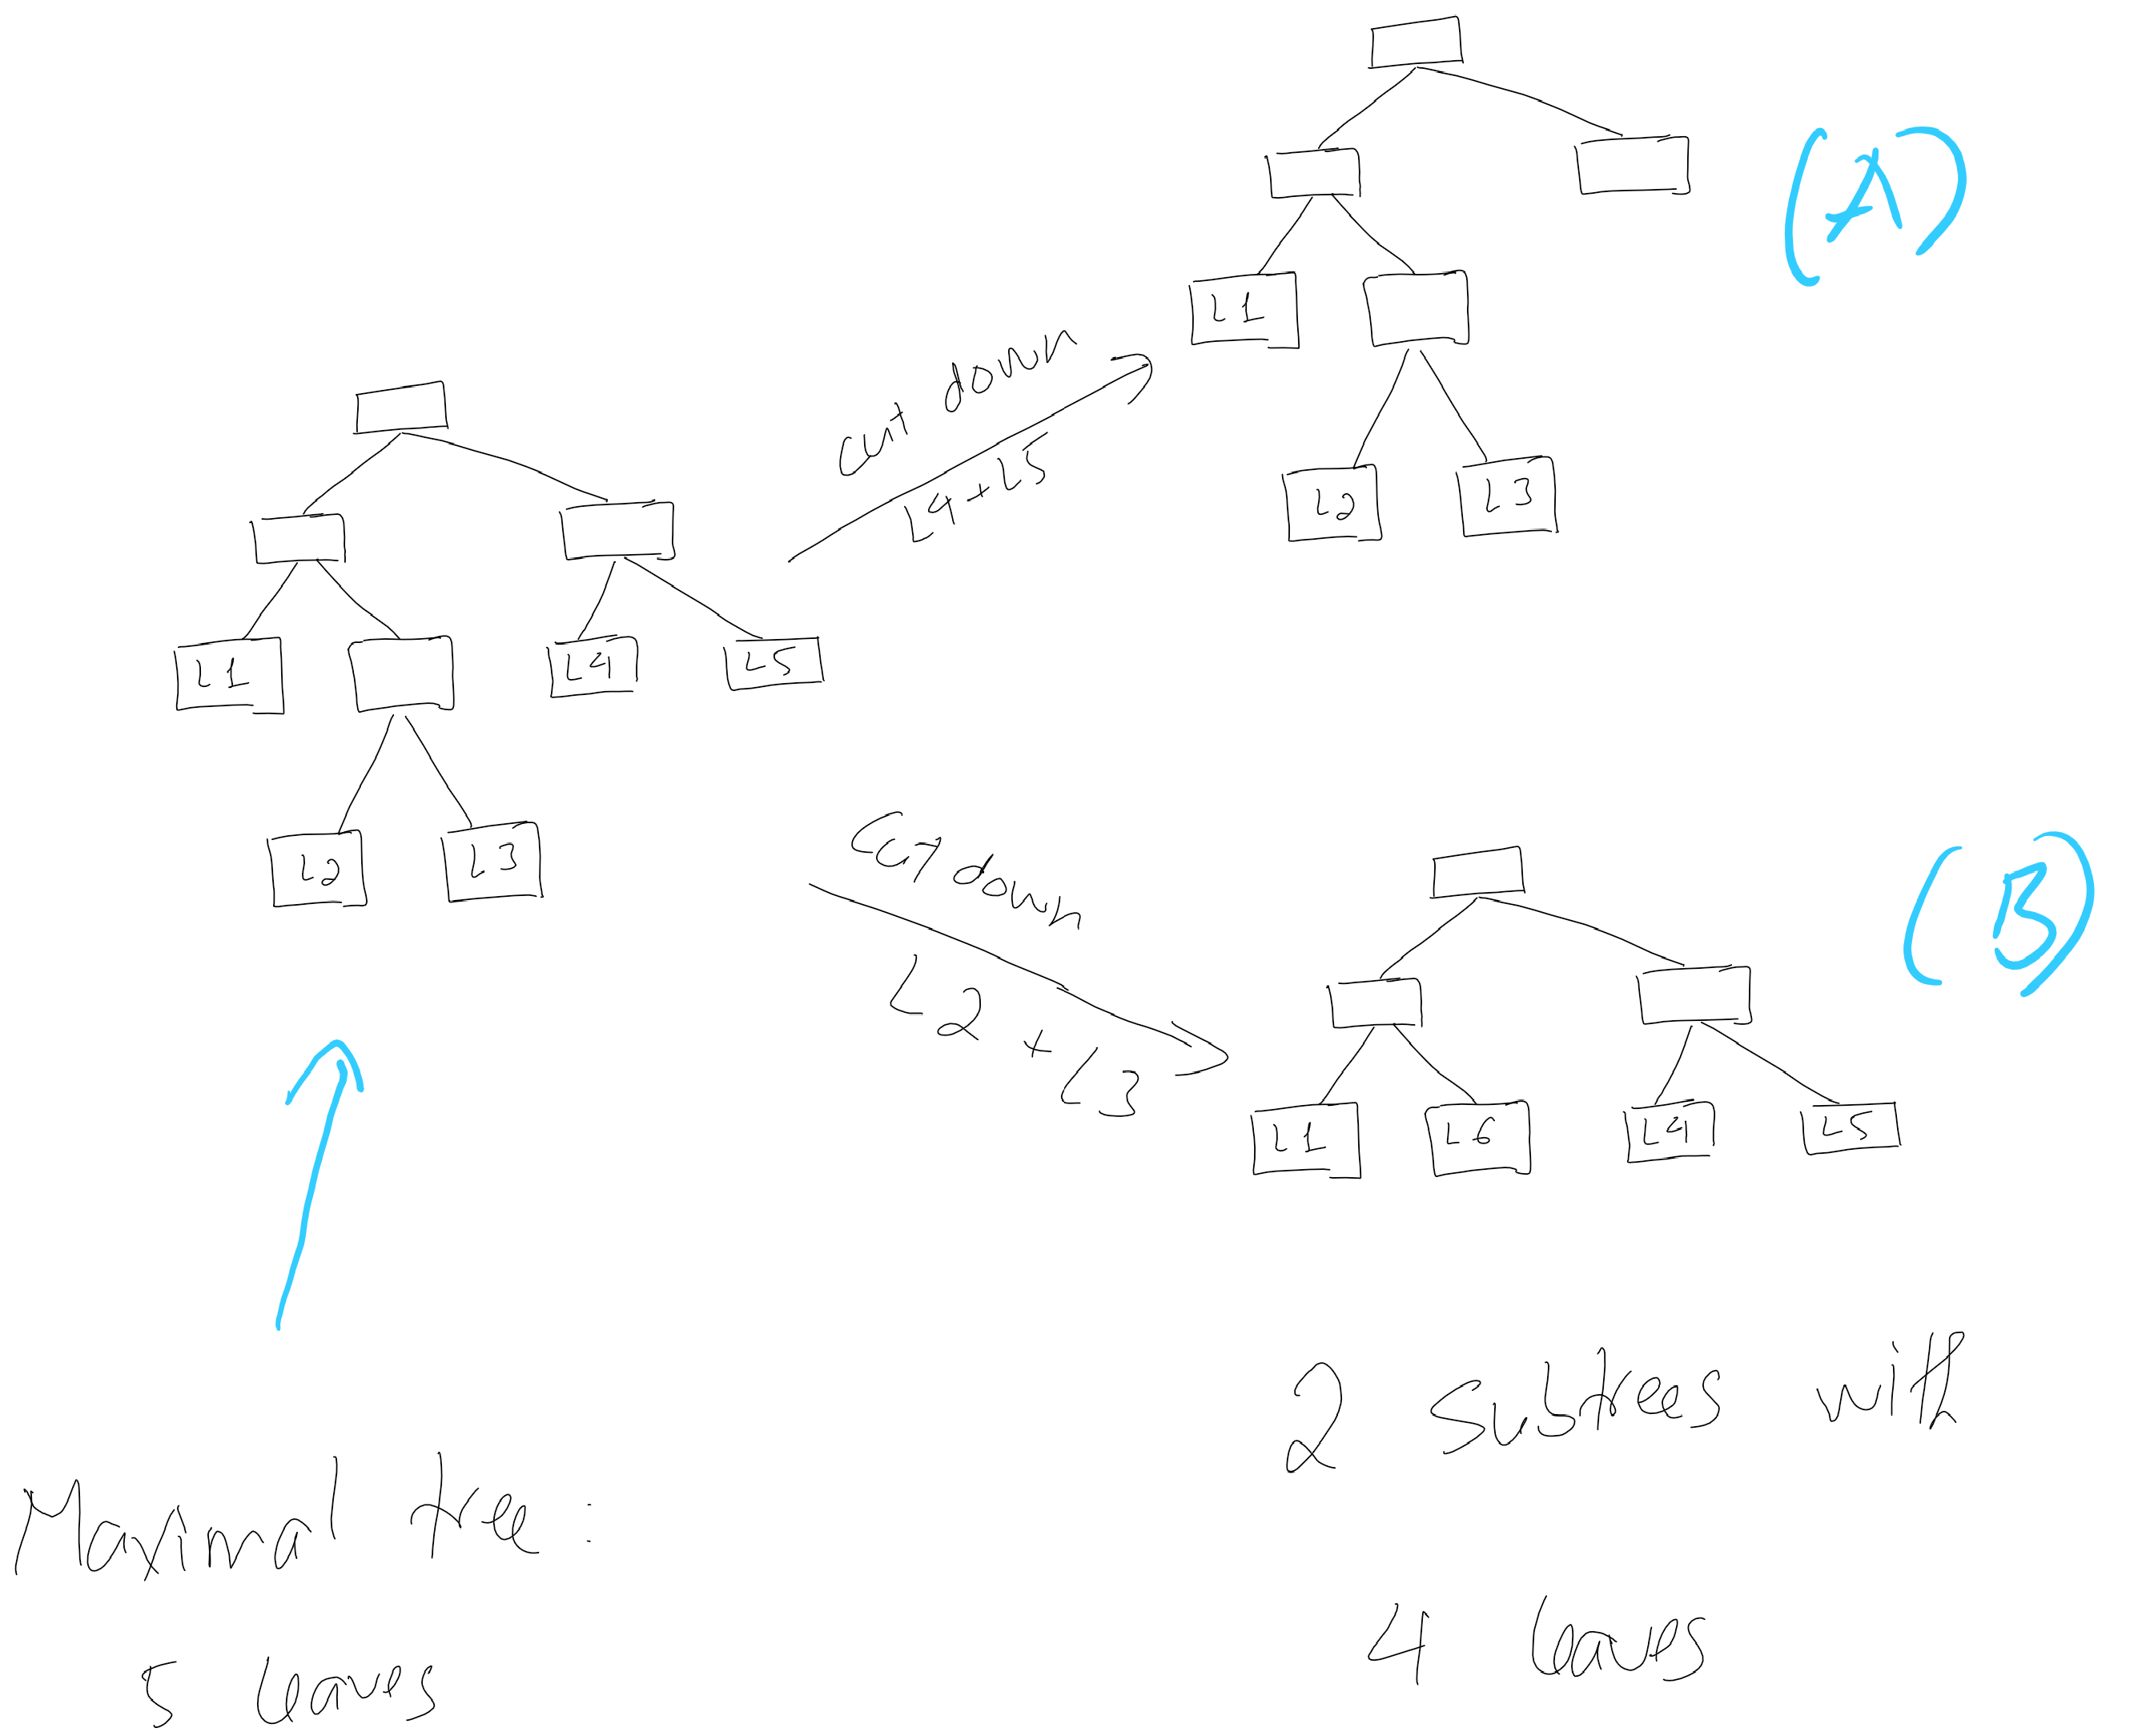
\includegraphics{images/tree8.png}
\end{frame}

\begin{frame}{Example of Tree Prunning}
\phantomsection\label{example-of-tree-prunning-1}
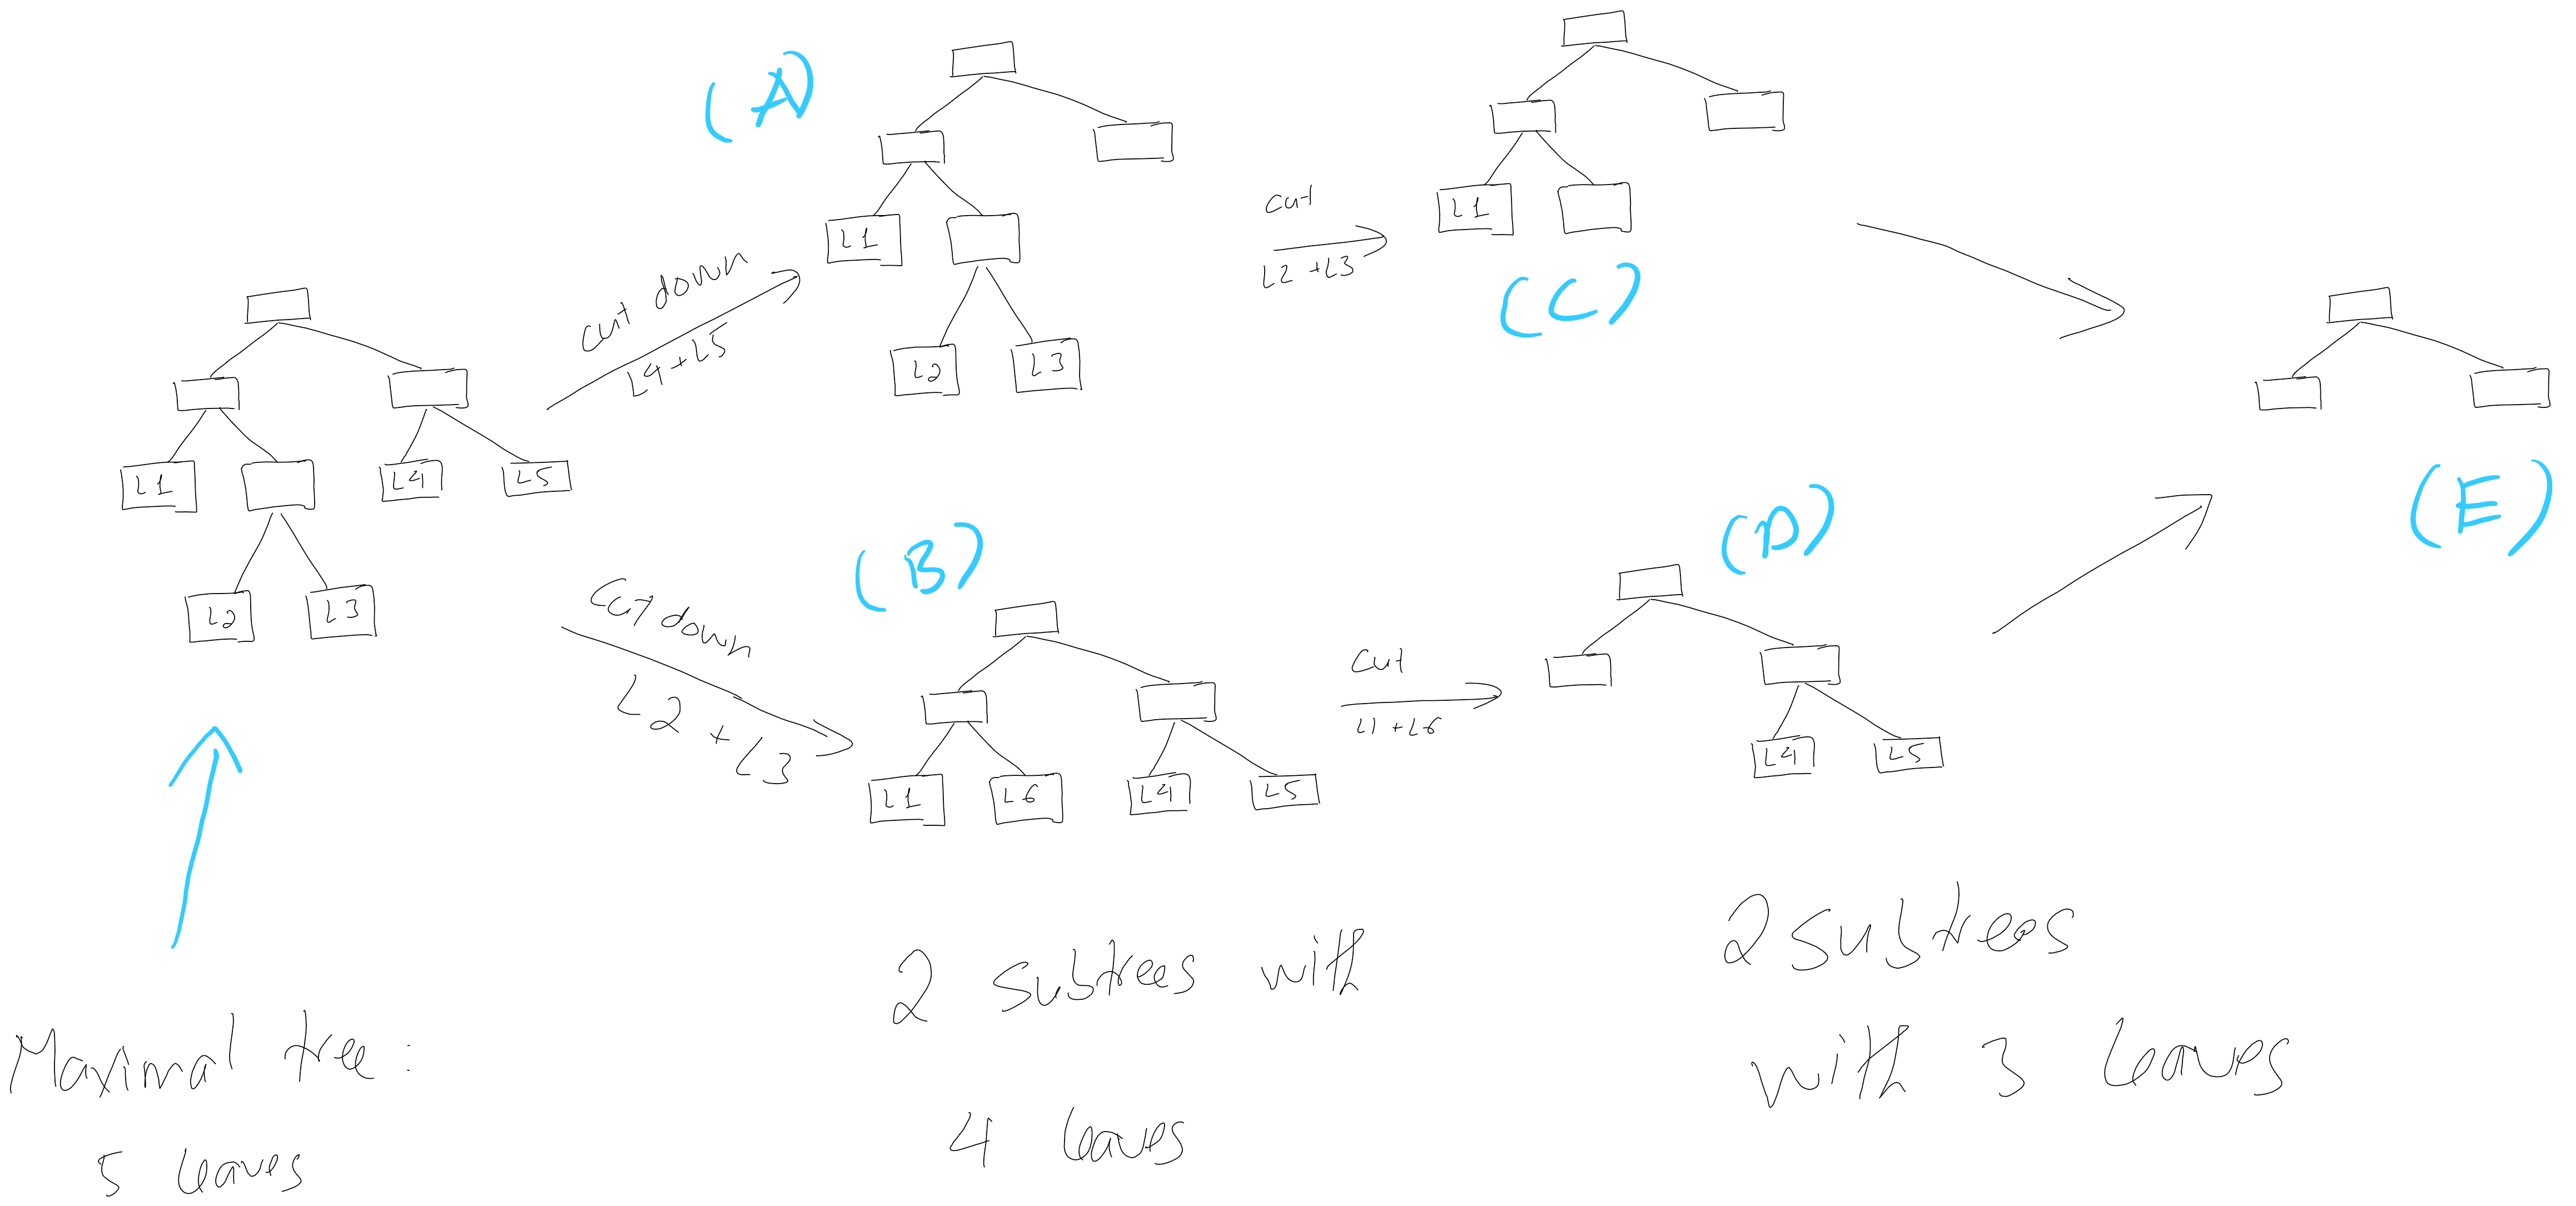
\includegraphics{images/tree9.png} - All the subtrees A, B, C, D, and E
will be validated with the validation data to find the \textbf{optimal
tree} - The \textbf{optimal tree} could be the \textbf{maximal tree}!
\end{frame}

\begin{frame}{Question}
\phantomsection\label{question-1}
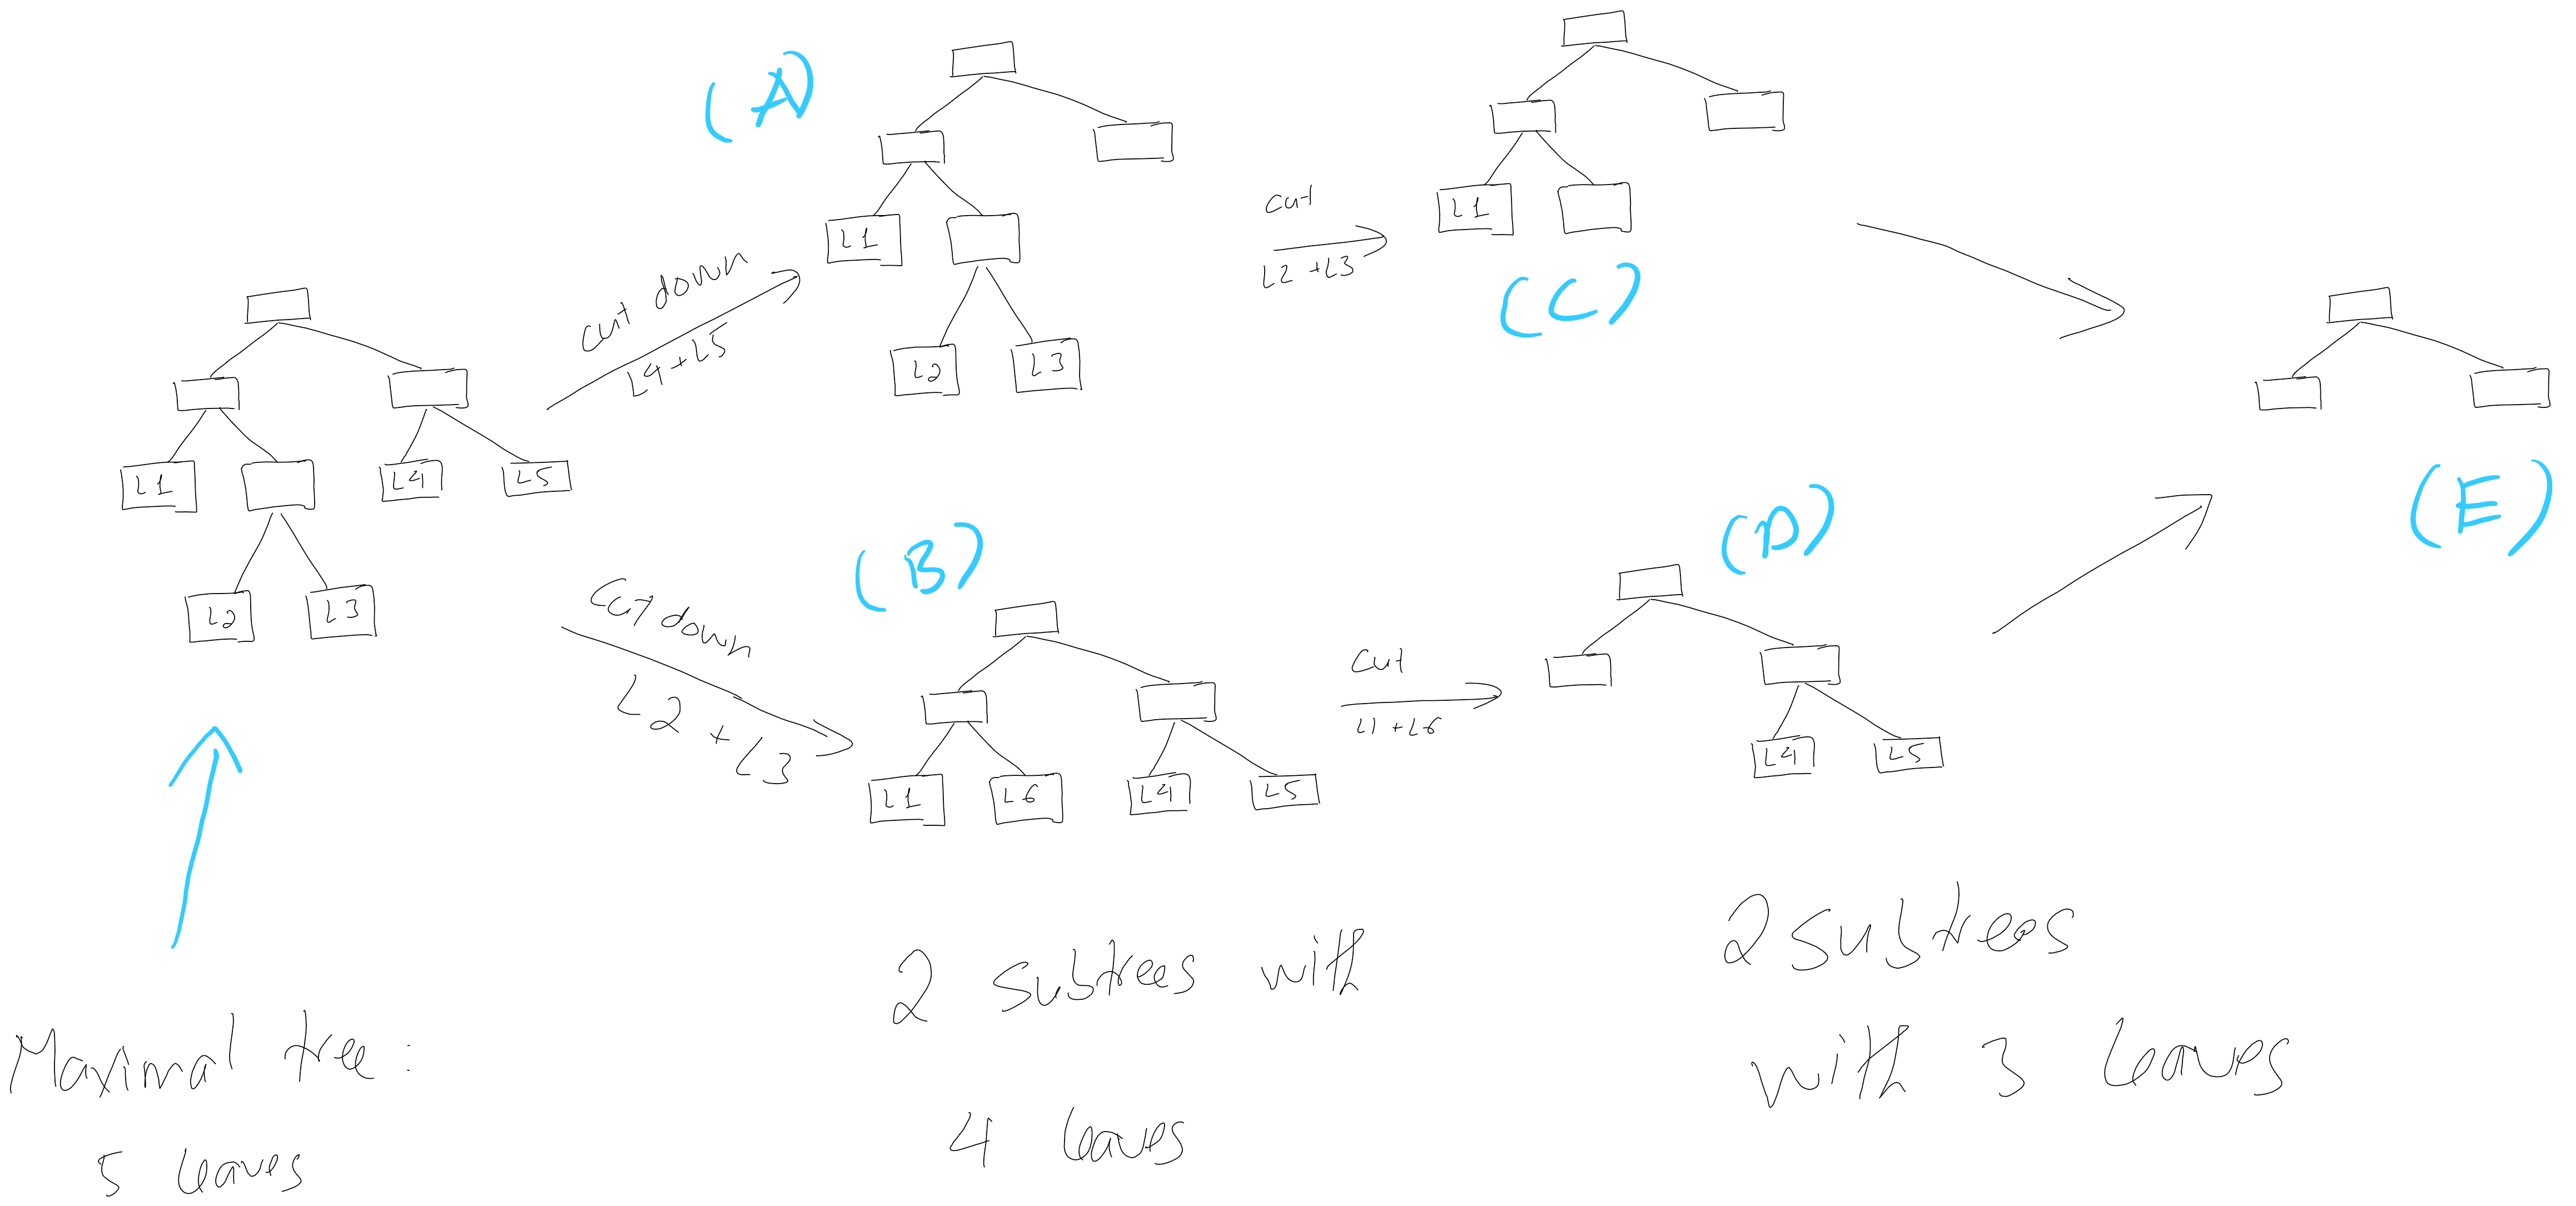
\includegraphics{images/tree9.png} - What if both B and C give the
lowest error on the validation data? Which tree should be selected as
the final model?
\end{frame}



\end{document}
